\chapter{计算机系统概述}

\section{操作系统的基本概念}

\subsection{操作系统的概念}

    \emph{操作系统(Operator System)是指控制和管理整个计算机系统的{\color{red}硬件和软件资源},合理地组织、调度计算机的工作与资源的分配,进而为用户和其他软件提供方便接口与环境的程序集合。}

    \emph{\color{red}操作系统是计算机系统中最基本的系统软件。}

\subsection{操作系统的特征}

    操作系统有如下四大特征:

\begin{itemize}
    \item [1.] 并发(Concurrence)
    \subitem 并发是指两个或多个事件在同一时间间隔内发生。值得注意的是:\emph{并发和并行是两个不同的概念,{\color{red}并行一定并发,并发不一定并行。对于单处理器来说,只能并发执行。}}
    \subitem \emph{并发是OS最为基础且必要的特征。}
    \item [2.] 共享(Sharing)
    \subitem 共享即资源共享,是建立在并发之上的。
    \subitem (互斥式共享) 系统中的某些资源在一个时间段内有且仅能一个程序进行访问和操作,且把\emph{{\color{red}该资源称为临界资源。}}
    \subitem (同时式共享) 该类资源可以由多个程序同时段进行访问(多出现在读操作上)
    \subitem \emph{并发和共享是操作系统{\color{red}最基本}的特征,两者之间互为存在的条件:资源共享必定是由并发产生的,而共享影响了并发则会导致并发崩溃。}
    \item [3.] 虚拟(Virtual)
    \subitem \emph{虚拟是指把一个物理上的实体变为若干逻辑上的对应物。{\color{red}物理实体是实际存在的,而虚拟逻辑是用户感觉上的事物。}}
    \subitem 虚拟处理器的存在:时分复用技术
    \subitem 虚拟内存的存在:空分复用技术
    \item [4.] 异步(Asynchronism)
    \subitem 多道程序环境允许多个程序执行,但由于资源有限(竞争的情况),进程并非一贯到底的执行。而且走走停停,不停的切换,因此以不可预知的速度向前推进。
\end{itemize}

\subsection{操作系统的目标与功能}

    \emph{为了给多道程序提供环境,OS应该具备:处理机(进程)管理、存储器(内存)管理、设备管理和文件管理(现代操作系统中,不仅仅这几个模块)。}

    \emph{除了上述的模块外,还需要提供各种接口。}

\subsubsection{操作系统作为计算机系统资源的管理者}

\begin{itemize}
    \item [1)] 处理机(进程)管理
    \subitem 在多道程序环境下,处理机的分配和运行都以进程(或线程)为基本单位,因此对处理机管理可归结为进程管理。
    \subitem 并发指的是\emph{计算机内同时运行多个进程,因此如何管理进程则是最主要的任务。进程管理的主要功能包括进程控制、进程同步、进程通信、死锁处理、处理机调度等。}
    \item [2)] 存储器(内存)管理
    \subitem 内存管理是为了给多道程序的运行提供良好的环境,方便用户使用以及提高利用率。\emph{其主要包括内存分配与回收、地址映射、内存保护与共享和内存扩充等。}
    \item [3)] 文件管理
    \subitem \emph{{\color{red}计算机中的信息都是以文件的形式存在的},文件管理包括文件存储空间的管理、目录管理以及文件读写管理与保护等。}
    \item [4)] 设备管理
    \subitem 设备管理的主要任务是完成用户的I/O请求,方便用户使用各种设备,提高设备利用率。主要包括缓冲管理、设备分配、设备处理和虚拟设备等。
\end{itemize}

\subsubsection{操作系统作为用户与计算机硬件系统之间的接口}

\begin{itemize}
    \item [1)] 命令接口
    \subitem (联机命令接口(交互式)) \emph{{\color{red}适用于分时或实时操作系统。}由一组键盘命令组成,用户通过控制台或terminal输入命令与OS进行交互。}类似于Python交互器。
    \subitem (脱机命令接口(批处理)) \emph{{\color{red}适用于批处理系统。}由一组作业控制命令组成,不能直接干预作业的运行,事先使用对应的作业控制命令写成一份操作流程,然后递交给OS。}类似于Bash脚本。
    \item [2)] 程序接口
    \subitem 程序接口由系统调用(又称广义指令)组成,例如printf、malloc等C语言调用接口。
    \subitem GUI就是图形接口,其最终是通过调用程序接口实现的。{\color{red}严格的说,GUI不是操作系统的一部分,但GUI所使用的系统调用是OS的一部分。}
\end{itemize}

\subsubsection{操作系统实现了对计算机资源的扩展}

    \emph{没有{\color{red}任何软件支持的}计算机被称为裸机,其仅构成计算机系统的物质基础。}

    也就是说,操作系统的内部是各种物理结构所组成的逻辑环境,操作系统所提供的资源管理功能和方便用户的各种服务功能,将裸机改造成功能更强、更方便的机器。\emph{通常,把覆盖了软件的机器称为扩充机器或虚拟机。}

\section{操作系统发展历程}

\subsection{手工操作系统}

    \emph{此阶段并未产生严格意义上的OS。} 

    手工操作系统的突出缺点:\emph{用户独占全机,资源利用效率极低;CPU等待手工操作,CPU利用效率极低。}

\subsection{批处理阶段}

    \emph{为了解决人机矛盾以及I/O设备之间速度不匹配的问题,出现了批处理系统。}

\subsubsection{单道批处理系统}

    系统对作业的处理是成批进行的,但{\color{red}内存中始终只保存一道作业。}其主要特征为:

\begin{itemize}
    \item [1)] 自动性。磁带上的一批作业自动逐个进行,无需人工干预
    \item [2)] 顺序性。磁带上的作业按顺序进入内存
    \item [3)] 单道性。内存中仅有一道作业运行,即监督程序每次从磁带上只调入一道程序。
\end{itemize}

    单道批处理系统的主要问题在于:\emph{内存中仅有一道作业,CPU有大量的时间是在等待I/O的完成。}

\subsubsection{多道批处理系统}

    为了解决资源利用率和系统吞吐量,引入了多道程序技术。\emph{多道程序技术允许多个程序同时进入内存并允许在CPU中交替运行,共享系统中的各种软硬件资源。}

    其设计的特点为\emph{多道、{\color{red}宏观上并行,微观上串行。}}但是,多道程序设计需要解决:

\begin{itemize}
    \item [1)] 如何分配处理器
    \item [2)] 如何分配内存
    \item [3)] 如何分配I/O设备
    \item [4)] 如何组织和存放大量的程序和数据,且保证数据安全和一致性
\end{itemize}

    其优点在于:\emph{资源利用率高,且共享计算机资源从而使各种资源得到充分利用;系统吞吐量大,CPU和其他资源保持“忙碌”状态。}

    缺点在于:\emph{用户响应时间较长;不提供人机交互能力,用户既不能了解运行情况也不能控制计算机。}

\subsubsection{分时操作系统}

    \emph{分时技术,也就是将处理器的运行时间分成很短的时间片,按照时间片轮流把处理器分配给各联机作业使用。{\color{red}这使得每个用户(程序)感觉起来就像自己独占一台计算机}。}

    \emph{分时操作系统,指的是多个用户通过终端同时共享一台主机,用户可以同时与主机进行交互操作而互不干扰。}因此,分时系统最关键的问题在于:{\color{red}如何使用户与自己的作业交互}。分时系统支持多道程序设计,但不同于多道批处理,分时系统是人机交互的系统:

\begin{itemize}
    \item [1)] 同时性。\emph{同时性又称多路性,允许多个终端用户同时使用一台计算机。}
    \item [2)] 交互性。用户能够与系统进行人机对话。
    \item [3)] 独立性。系统中的各个用户独立操作,互不干扰。
    \item [4)] 及时性。用户请求能在很短时间内响应,采用时间片轮转算法。
\end{itemize}

\subsubsection{实时操作系统}

    \emph{为了满足某个时间限制内完成某些紧急任务而不需要时间片排队,诞生了实时操作系统。}

    硬实时系统:\emph{某个动作必须绝对地在规定的时刻内完成或发生。}

    软实时系统:\emph{能够接收偶尔违反时间规定且不会引起任何永久性的损害。}

    在实时操作系统的控制下,计算机系统接收到外部信号后及时处理,并在严格时间内处理完毕,其主要特点就是{\color{red}及时性和可靠性}。

\section{操作系统运行环境}

\subsection{处理器运行环境}

    在OS中,CPU通常执行两种不同性质\footnote[1]{\emph{就我所知,现代OS中的等级应该大多数是三级,M、S、U,分别表示机器级、监管者、用户级。}}的程序:一种是OS Kernel程序;一种是User program。对于OS来说,前者是后者的管理者,管理程序需要执行一些特权指令,而用户程序出于安全考虑不允执行。

    同时,OS中将程序的环境分成了两态,分别对应了{\color{red}特权级的内核态}以及{\color{red}非特权级的用户态}\footnote[1]{在OS中,一般会存在一个特殊寄存器PSW(程序状态字寄存器),主要用于判断当前运行环境是内核态还是用户态。},其用于用户程序和内核程序不同运行的环境。

\begin{itemize}
    \item [1)] 特权指令,\emph{指的是不允许用户直接使用的指令,比如I/O指令,置中断指令等一系列需要内核态环境下完成的指令。}
    \item [2)] 非特权指令,\emph{指的是允许用户直接使用的指令,不能直接访问系统中的软硬件资源,仅限于访问用户的地址空间。}
\end{itemize}

    需要注意的是:\emph{{\color{red}OS中的内核态和用户态是不断切换的,以适应不同的需求。}}如果想要从内核态切换到用户态,那么直接使用对应的特权指令进行“降级操作”(例如在rv架构上的sret指令)。如果需要从用户态切换到内核态,那么必须通过中断操作(\emph{{\color{red}此处的中断是广义的,包括了狭义的中断和异常}}),触发中断信号,{\color{red}硬件自动完成变态操作}。

    内核是计算机上配置的底层软件,管理了系统的各种资源:

\begin{itemize}
    \item [1.] 时钟管理
    \subitem \emph{\color{red}在计算机的各部件中,时钟是最为关键的设备}。时钟的第一功能是计时,OS通过时钟管理来获取标准的系统时间,且通过时钟中断实现进程的切换。
    \item [2.] 中断机制
    \subitem 引入中断的初衷是为了提高多道程序运行环境中CPU的利用率。就目前来说,\emph{\color{red}现代操作系统就是靠中断驱动的软件}。
    \subitem \emph{中断机制中,仅有一小部分属于内核,负责保护和恢复终端现场信息,转移控制权到相关的处理程序}。
    \item [3.] 原语
    \subitem \emph{操作系统提供的基本操作接口或函数,用于实现高级操作系统功能和管理底层资源。原语通常是操作系统内核的一部分,提供了对硬件和系统资源的底层访问和控制。}
    \begin{itemize}
        \item [1)] 处于OS的最底层,是最接近硬件的部分
        \item [2)] 具有原子性,其操作只能一气呵成
        \item [3)] 运行时间短,调用频繁 
    \end{itemize}
    \subitem 定义原语的直接方法是关闭中断,让其所有动作不可分割地完成后再打开中断。
    \item [4.] 数据结构及处理
    \subitem 在OS中,定义了很多登记状态的数据结构,如作业控制块、进程控制块(PCB)、设备控制块、各种链表、队列等。常见的为三种:
    \begin{itemize}
        \item [1)] 进程管理。进程状态、调度与分派、创建、撤销等
        \item [2)] 内存管理。内存分配回收、保护、对换等
        \item [3)] 设备管理。缓冲区、设备分配、回收等
    \end{itemize}
\end{itemize}

\subsection{中断和异常的概念}

\begin{quote}
    \emph{OS引入内核态和用户态后,必须考虑的事情就是如何切换,如何留下“门”。}
\end{quote}

\subsubsection{中断和异常的定义}

    中断(Interruption)也叫做外中断,\emph{指的是来自CPU执行指令外部的事件,通常用于信息输入/输出,例如I/O中断,时钟中断等。}

    异常(Exception)也叫做内中断,\emph{指的是CPU执行指令内部的事件,例如非法操作、越界、缺页或trap指令。}值得注意的是,{\color{red}异常不能被屏蔽,一旦出现,需要立刻处理。}

\begin{figure}[!htbp]
    \centering
    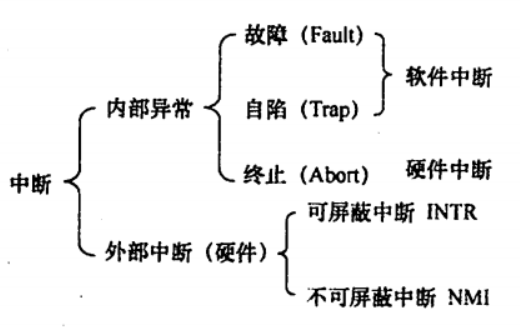
\includegraphics[width=0.6\textwidth]{image/chapter01/异常和中断区分.png}
    \caption{中断和异常的联系与区别}
\end{figure}

\subsubsection{中断和异常的分类}

    外中断可分为可屏蔽中断和不可屏蔽中断。\emph{可屏蔽中断通过INTR线发出中断请求,通过改变屏蔽字可以实现多重中断;不可屏蔽中断通过NMI线发出中断请求,一般比较紧急,因此不可屏蔽}。

    异常分为故障、自陷(trap)和终止。故障(Fault)通常由指令引起的异常,如非法操作码,缺页异常,除零等;自陷(Trap)是一种实现安排的“异常”行为,用户通过自陷操作从而进入内核态执行特权代码。终止(Abort)指出现了使CPU无法继续执行的硬件故障。

    \emph{故障异常和自陷异常属于软中断,外部中断和终止异常属于硬中断。}

\subsubsection{中断和异常的处理}

\begin{itemize}
    \item [1.] 当CPU运行时检测到异常事件(或检测到一个中断请求信号)
    \item [2.] 保存现场状态
    \item [3.] CPU打断当前执行,通过中断(异常)信号,查询中断向量表,跳转到对应的中断或异常处理程序
    \item [4.] 若能处理,则返回执行,恢复现场;若不能处理,终止程序
\end{itemize}

\subsection{系统调用}

    \emph{用户在程序中调用OS所提供的一些子功能,系统调用可被视为特殊的公共子程序。}

    \emph{系统中的各种共享资源都是由OS统一管理},因此,\emph{OS为了安全以及稳定起见,统一的为用户提供了接口,使得用户只要涉及资源相关的操作,就必须通过系统调用来提出服务请求,由OS来代理完成。}

\begin{itemize}
    \item 设备管理。完成设备的请求和释放,以及设备的启动等
    \item 文件管理。完成文件的读写、创建、删除等
    \item 进程管理。完成进程的创建、删除、阻塞等
    \item 进程通信。完成进程之间信息的传递等
    \item 内存管理。完成内存的分配、回收等
\end{itemize}

    那么,对于上述的操作,其内部肯定是需要在内核态中运行一些特权指令的,因此,系统调用就需要用用户态切换到内核态去执行。因此,OS提供了特殊的trap指令来发起系统调用请求。

    也就是说,OS的运行环境就可以为:用户通过OS运行上层应用,其依赖于OS的底层管理程序提供服务支持,当需要管理程序服务时,则通过中断(异常)机制进入内核态,运行管理程序。同时,在进入内核态时,需要保存现场。

\begin{figure}[!htbp]
    \centering
    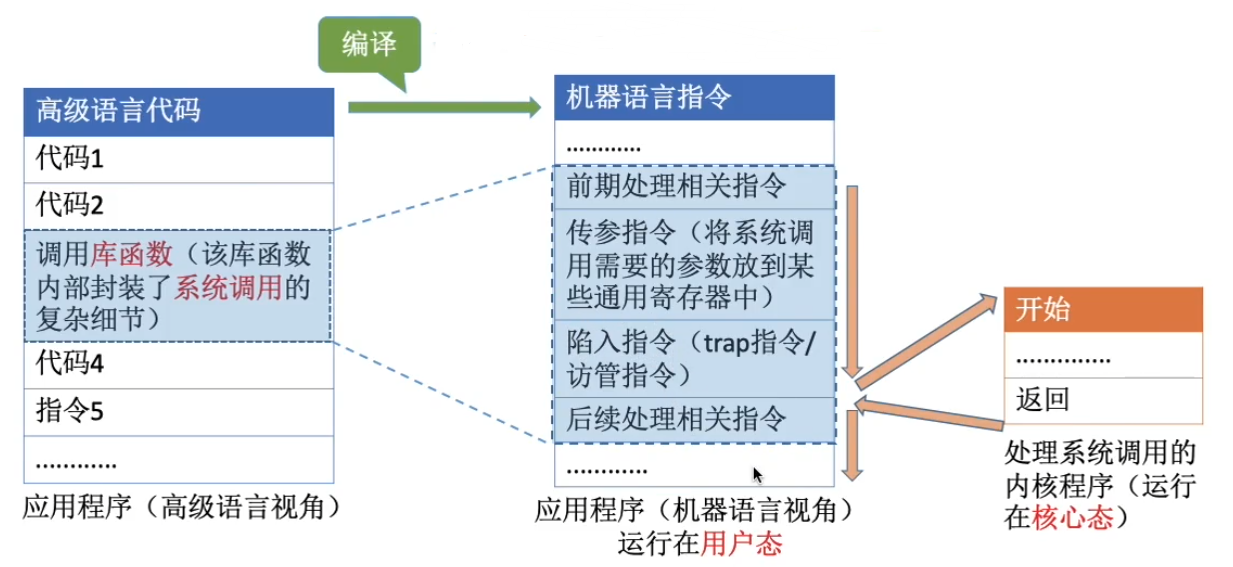
\includegraphics[width=0.8\textwidth]{image/chapter01/系统调用过程.png}
    \caption{系统调用的过程}
\end{figure}

    值得注意的是:

    \emph{1. 陷入指令是在用户态执行的,会立即产生一个软中断,使CPU进入内核态。}

    \emph{2. 发出的系统调用请求在用户态,执行在内核态(通过传参指令,告诉系统调用入口程序要调用哪一个系统调用)。}

\section{操作系统结构}

\subsection{分层法}

    分层法是将操作系统分为若干层,最底层是硬件,最高层是用户接口,\emph{\color{red}每层只能调用紧邻的低层的功能和服务(单项依赖)}。

\begin{figure}[!htbp]
    \centering
    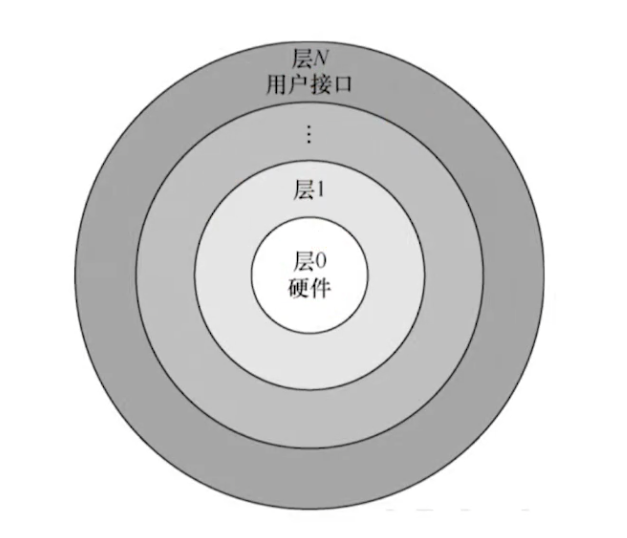
\includegraphics[width=0.4\textwidth]{image/chapter01/分层法.png}
    \caption{分层法系统}
\end{figure}

    分层法的优点:\emph{1. 便于系统的调试和验证,简化了系统的设计和实现;2. 易扩充和已维护,只需要逐层验证,且保证上下层接口即可轻易的扩充和修改。}

    分层法的缺点:\emph{1. 合理定义各层困难,需要考虑固定的依赖关系;2. 效率差,由于只能一层层的传递,因此每层都需要通信机制,而通信机制又会带来额外的开销,在分层法中尤为突出。}

\subsection{模块化}

    \emph{就目前来说,模块化是主流OS必不可少的机制。}

    模块化是将\emph{OS按功能划分为若干具有一定独立性的模块,每个模块具有某方面的功能,并规定好接口使之能互相通信。}

\begin{figure}[!htbp]
    \centering
    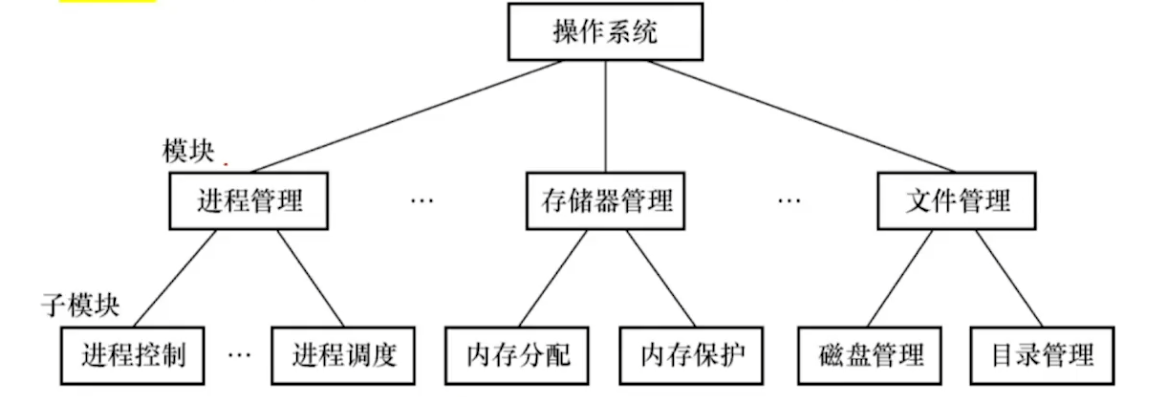
\includegraphics[width=0.6\textwidth]{image/chapter01/模块化.png}
    \caption{模块化系统结构}
\end{figure}

    模块化的划分是一件困难的事情,若划分太小,则各模块之间的耦合度过高;若太大,模块内部的复杂性过高。同时,还需要考虑到模块的独立性,越高,各模块之间的交互就越少,结构就越清晰。衡量模块的独立性主要为:

\begin{itemize}
    \item 内聚性。模块内部各部分间联系的紧密程度,内聚性越高,独立性越好
    \item 耦合度。模块间相互联系和相互影响的程度,耦合度越低,独立性越好
\end{itemize}

    模块化的优点:\emph{1. 提高了OS设计的正确性、可理解性和可维护性;2. 增强了OS的可适应性;3. 加速了OS的开发过程;4. 支持动态的增加模块功能}

    模块化的缺点:\emph{1. 模块间的接口规定难以满足对接口的实际需求;2. 各模块设计者共同开发,水平层次不齐,无法建立在上一个正确决定的基础上}

\subsection{宏内核}

    \emph{主流OS的选择。}

    宏内核,也称单内核或大内核,\emph{指的是将OS的主要功能模块都作为一个紧密联系的整体运行在内核态,从而为用户程序提供高性能的系统服务。}

    因为各模块间共享信息,能有效利用互相之间的有效特性,所以具有无可比拟的性能优势。

    不过,就目前来说,\emph{例如Linux,目前的瓶颈就在于宏内核使得代码量冗余,且无法有效的拆分(哪怕是运用了模块化的机制),导致内核功能复杂,难以维护。且内核中若某个重要模块出错,则会导致整个系统崩溃。}

\subsection{微内核}

    微内核架构,\emph{指的是将内核中最基本的功能保留在内核,其余功能移交到用户态执行,从而降低内核的设计复杂性。且同时本身具有模块化的机制,也就是将移出内核的模块按照分层的原则划分为若干服务程序,执行互相独立,交互借助于微内核通信。}

    微内核结构将OS分为了两块:微内核和多个服务器。微内核是精心设计的、实现OS最基本核心功能的小型内核,其只包括了:\emph{1. 与硬件相关的部分;2. 原语操作;3. 通信功能。}其他类似于,进程管理、文件管理等则作为一个个服务模块与微内核进行通信。

\begin{figure}[!htbp]
    \centering
    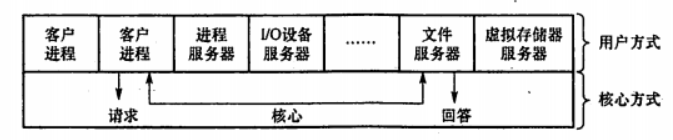
\includegraphics[width=0.8\textwidth]{image/chapter01/单机下的微内核模式.png}
    \caption{单机模式下的微内核模式}
\end{figure}

    为了提高可靠性,微内核架构中只有微内核运行在内核态,其他模块均在用户态,需要通信时,必须借助于微内核;同时,模块的错误只会导致模块崩溃,不会影响到微内核的运行。

    微内核所提供的基本功能:

\begin{itemize}
    \item [1)] 进程(线程)管理。进程(线程)之间的通信是微内核最基本的功能,同时还有切换、调度等。{\color{red}对进程的分类,优先级则是属于策略,应当放入进程管理服务器中}。
    \item [2)] 低级存储器管理。微内核中只配置了类似于逻辑地址转换物理地址的页表机制和变换机制这种依赖硬件的功能。至于页表置换等策略,部署在存储器管理服务器中。
    \item [3)] 中断和陷入处理。
\end{itemize}

    微内核的特点:\emph{1. 扩展性和灵活性;2. 可靠性和安全性;3. 可移植性;4. 分布式计算}

    微内核的缺点:\emph{{\color{red}最致命的,也就是主流OS不选择微内核的问题就是,效率过低,由于模块间会不断的通信,因此会在用户态和内核态频繁切换,执行开销过大。}}

\subsection{外核}

    OS外核(Exokernel)是一种操作系统设计模式,\emph{它的目标是提供最小化的内核功能,将更多的控制权和灵活性交给应用程序。在外核模式下,内核的功能被精简为最基本的硬件抽象和资源分配,而应用程序可以直接访问和控制底层硬件资源。}

\begin{figure}[!htbp]
    \centering
    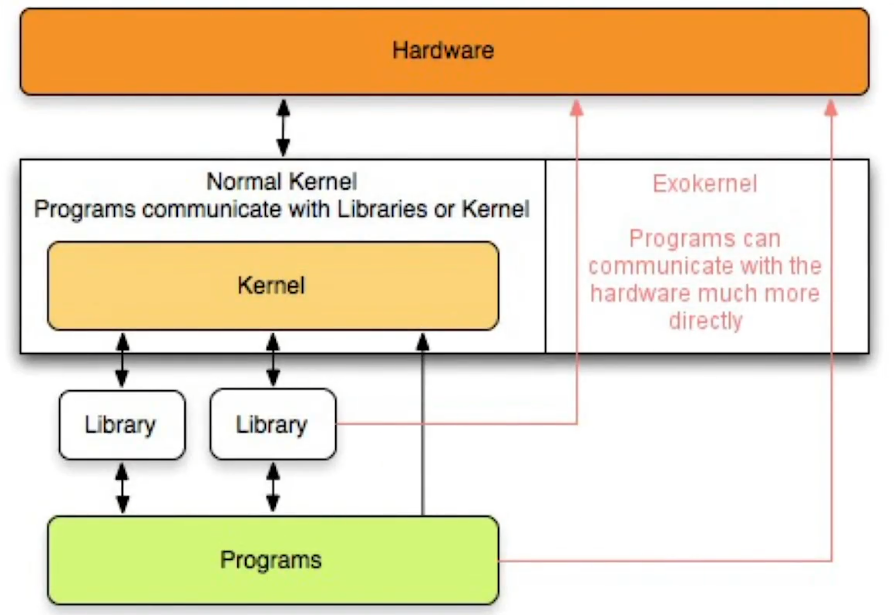
\includegraphics[width=0.6\textwidth]{image/chapter01/外核结构.png}
    \caption{外核结构}
\end{figure}

    \emph{外核{\color{red}只提供了硬件资源的抽象核保护机制,直接将底层硬件资源暴露}给应用程序,应用程序根据需求和策略进行资源分配、调度和优化。}

    外核模式的优势在于提供了更高的性能和灵活性。但是增加了开发和维护的复杂性。

\section{操作系统引导}

    OS是一种程序,程序以数据的形式存放在磁盘中,而硬盘分为多个区。OS引导是指\emph{计算机利用CPU运行特定程序,通过程序识别硬盘,识别硬盘分区,识别OS,最后启动。}

\begin{figure}[!htbp]
    \centering
    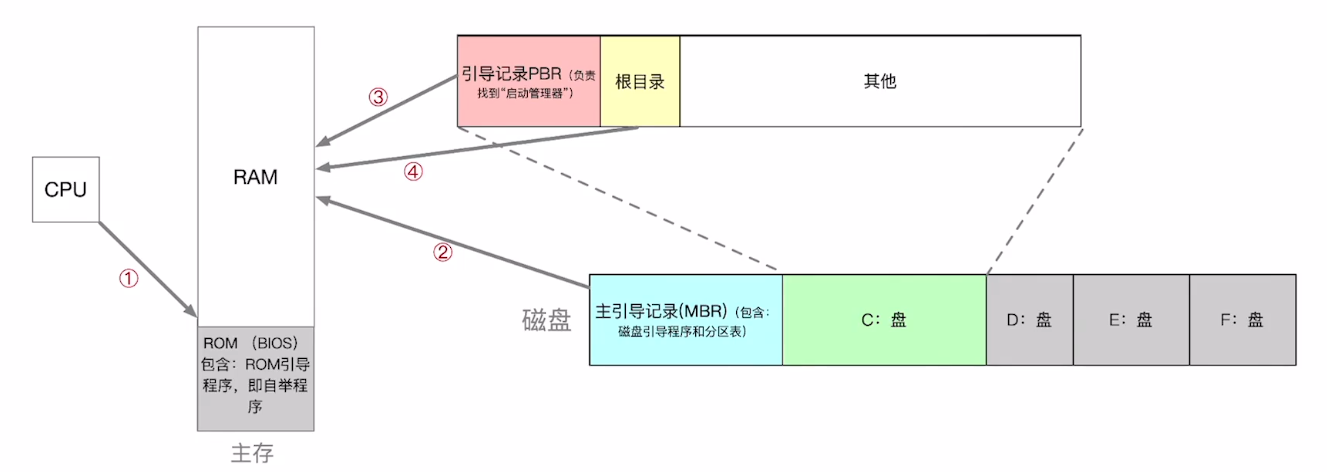
\includegraphics[width=0.8\textwidth]{image/chapter01/操作系统引导.png}
    \caption{操作系统引导过程}
\end{figure}

\begin{itemize}
    \item [1)] 激活CPU。CPU读取ROM中的Boot程序,将指令寄存器置为BIOS的第一条指令
    \item [2)] 硬件自检。BIOS首先会对硬件进行检查。
    \item [3)] 加载带有OS的硬盘。BIOS读取BootSequence(CMOS中的启动顺序,或用户交互),把控制权交给启动顺序排第一位的存储设备,然后加载该扇区内容。
    \item [4)] 加载主引导程序MBR。硬件以特定的标识符区分引导硬盘和非引导硬盘。主引导MBR的作用是告诉CPU去硬盘的哪个分区找到OS。
    \item [5)] 扫描硬盘分区表,并加载硬盘活动分区(含有OS的分区)。硬盘以特定的标识区分活动分区和非活动分区。若找到,移交控制权。
    \item [6)] 加载分区引导记录PBR。读取活动分区的第一个扇区,其作用是寻找并激活分区根目录下用于引导OS的程序(启动管理器)
    \item [7)] 加载启动管理器。
    \item [8)] 加载OS
\end{itemize}

\section{虚拟机}

    虚拟机\emph{是一台逻辑计算机,指利用特殊的虚拟化技术,通过隐藏特定计算平台的实际物理特性,为空户提供抽象的、统一的、模拟的计算环境。}

\subsection{第一类虚拟机管理程序}

    \emph{注意,第一类VMM和双系统是两个截然不同的东西。}

    从技术上来说,\emph{第一类VMM就像一个OS,因为它是{\color{red}唯一一个运行在最高特权级的程序}。VMM向上提供若干虚拟机,这些虚拟机时逻辑硬件的精确复制品。}

\begin{figure}[!htbp]
    \centering
    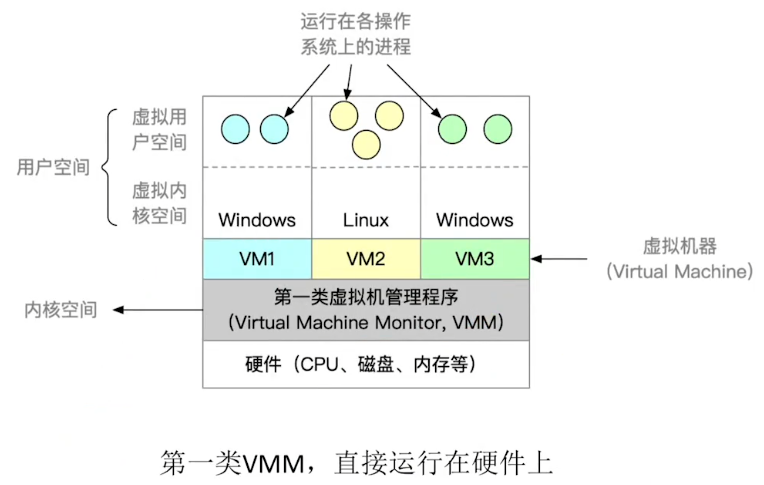
\includegraphics[width=0.6\textwidth]{image/chapter01/第一类VMM.png}
    \caption{第一类VMM}
\end{figure}

    虚拟机作为用户态的一个进程运行,不允许执行特权指令(因为虚拟机运行在用户态)。但是,\emph{由于虚拟机是一个完整的OS,因此它认为自身运行在内核态,称为虚拟内核态。因此,虚拟机内核态所执行的特权指令,会被转化为{\color{red}对VMM的调用请求}。}

\subsection{第二类虚拟机管理程序}

    \emph{第二类VMM就是我们所熟知的VMware、VMBox软件所虚拟的程序。}

    第二类VMM运行在OS上,就像一个普通的进程,同时,OS为在VMM上运行的虚拟OS提供各种虚拟资源。

\begin{figure}[!htbp]
    \centering
    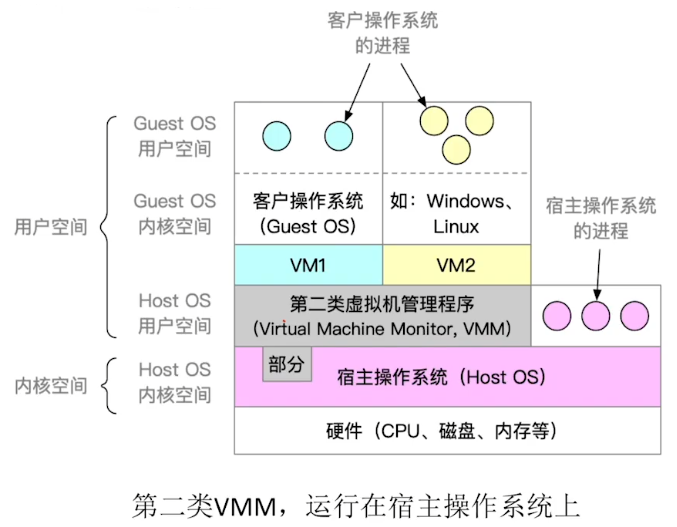
\includegraphics[width=0.6\textwidth]{image/chapter01/第二类VMM.png}
    \caption{第二类VMM}
\end{figure}

\subsection{区别与联系}

\begin{itemize}
    \item 对资源的控制权
    \subitem 第一类直接运行在硬件上,直接控制和分配;第二类运行在Host OS上,依赖于Host OS分配和管理
    \item 资源分配方式
    \subitem 第一类安装Guest OS时,VMM需要在原本的硬盘上自行分配存储空间;第二类拥有自己的虚拟磁盘,实际是Host OS文件系统上的一个大文件
    \item 性能
    \subitem 第一类性能优于第二类
    \item  可支持的虚拟机数量
    \subitem 第一类不需要和Host OS竞争资源,因此能够分配更多;第二类需要竞争,因此更少
    \item 可迁移性
    \subitem 第二类的迁移性优于第一类
    \item 运行模式
    \subitem 第一类VMM在最高优先级(Ring0);第二类VMM运行在用户态、部分运行在内核态(VM驱动程序)。Guest发出的系统调用会被VMM截获,转化为VMM对Host的调用请求
\end{itemize}

